% !Mode:: "TeX:UTF-8" 

\BiChapter{图表公式}{Figures,Tables and Equations}

论文写作过程中最重要的是{\hei 图、表、公式}等内容的编排。

%=========================================================================================
\BiSection{图}{Figures}

图~\ref{fig_ch2}~是用~Tikz~画的,Visio~画不出这么好看的图。
%
\begin{figure}[!ht]
\centering
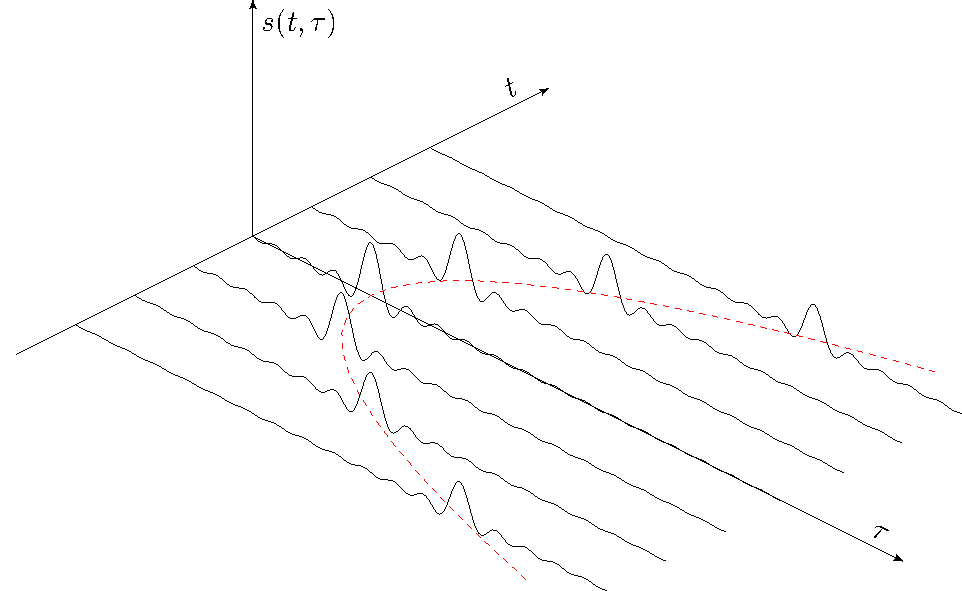
\includegraphics[width=\textwidth]{echoes}
\caption{图注是五号字。} \label{fig_ch2}
\end{figure}

%=========================================================================================
\BiSection{表}{Tables} 

表格要求采用三线表,如表~\ref{tab_ch2}~所示。
%
\begin{table}
	\renewcommand{\arraystretch}{1.2}
	\centering\wuhao
	\caption{表题也是五号字} \label{tab_ch2} \vspace{2mm}
	\begin{tabular}{c@{\hspace{1cm}}c@{\hspace{1cm}}c@{\hspace{1cm}}c}
	\toprule[1.2pt]
		Interference & DOA (deg) & Bandwidth (MHz) & INR (dB) \\
	\midrule[0.8pt]
		1 & $-30$ & 20 & 60 \\
		2 & 20 & 10 & 50 \\
		3 & 40 & 5 & 40 \\
	\bottomrule[1.2pt]
	\end{tabular}
\end{table}

%=========================================================================================
\BiSection{公式}{Equations}
\BiSubsection{单个公式}{Equations}

单个公式的编号如式~(\ref{equ_ch2_pdf})~所示,该式是标准正态分布的概率密度函数~\cite{Manolakis2005},从公式可知~\LaTeX~排版的公式比~MathType~美观,而且公式编写效率更高。
%
\begin{equation} \label{equ_ch2_pdf}
f_Z(z) = \frac{1}{\pi\sigma^2} \exp\left(-\frac{|z-\mu_Z|^2}{\sigma^2}\right)
\end{equation}

%-----------------------------------------------------------------------------------------
\BiSubsection{多个公式}{Subequations}

多个公式作为一个整体可以进行二级编号,如~(\ref{equ_ch2_fourier})~所示,该式是连续时间~Fourier~变换的正反变换公式~\cite{Vetterli2014}。
%
\begin{subequations} \label{equ_ch2_fourier}
\begin{align}
X(f) &= \int_{-\infty}^{\infty}x(t)e^{-j2\pi f t}\dif t \\
x(t) &= \int_{-\infty}^{\infty}X(f)e^{j2\pi f t}\dif f
\end{align}
\end{subequations}
